\section{Redes de comunicaciones moviles terrestres}
\subsection{Sistemas PMR y PMT}
\begin{itemize}
\item{PMR(Private Movil Radio):} Sistemas normalmente no conectados a la red telefónica pública conmutada que se modelan como sistemas de espera.
\item{PMT(Personal Movil Telecommunications):} Sistemas conectados a la red telefónica pública modelados como sistemas con pérdidas. 
\end{itemize}
\subsubsection{Private Movil Radio}
\label{ssub:PMR}
Las características que definen este sistema son las siguientes:
\begin{itemize}
	\item Tienen una area territorial limitada.
	\item No suelen estar conectados a la red telefónica pública conmutada(POTS).
	\item Se suelen usar para dar servicios de empresa como la gestión de flotas.
	\item Deben ser posibles tanto las llamadas entre estaciones moviles (MS) entre sí como las llamadas a grupos.
	\item Deben funcionar en regimen de espera con llamadas frecuentes y de corta duración.
	\item Lo normal es que funcionen en simplex pero hay casos de sistemas en semiduplex e incluso en full-duplex.
\end{itemize}
El ejemplo más representativo de los sistemas PMR es el sistema Trans European Trunked RAdio (TETRA). Dependiendo de como se asignen los canales de comunicación a los ususarios del sistema se puede distinguir entre los dos siguientes sistemas:
\begin{itemize}
	\item Asignación rígida: a un conjunto de ususarios se les asigna un único canal para la comunicación. Es un sistema de asignación bastante poco efectivo, por esto, se suele usar con colectivos relativamente pequeños.
	\item Asignación troncal: se tienen N canales que pueden ser usados por M usuarios.
\end{itemize}
l
\begin{example}[Sistemas PMR]
Se tiene un sistema PMR en el que los usuarios piden 1 llamada de 20 segundos por HC
\begin{gather*}
	\mu=\sfrac{1}{20}s^{-1}\\
	a_o=\frac{\lambda}{\mu}=\frac{20}{3600}=5.56mE	
\end{gather*}
\begin{center}
\begin{tabular}{|c|c|c|}
\hline
	N canales 	& Asignación fija 	& Asignación troncal \\\hline
	1 			& 21 				& 21 \\\hline
	2 			& 42 				& 125 \\\hline
	5 			& 105 				& 581 \\\hline
	10 			& 210 				& 1429 \\\hline
\end{tabular}
\end{center}
\begin{gather*}
0,05=C(1,A_O)e^{-\mu t(1-\rho)}=C(1,A_O)e^{-1+A_O}=A_Oe^{A_O-1} \to A_O=0,121E\\
M=\sfrac{A_O}{a}=21.7\to M=21\text{ móviles}
\end{gather*}
\end{example}
La cobertura de los sistemas PMR depende de la locaclización de las estaciones base (BS). En caso de que no sea necesaria una gran cobertura se utilizan sistemas monoemplazamiento. La red con cobertura monoemplazamiento está formada por un nodo central de control y su BS. Una red Multiemplazamiento, en cambio, está concebida para zonas de gran extensión cubierta por varios nodos interconectados. En este esquema habrá un nodo central de control. En los sistemas multiemplazamiento PMR  el traspaso no está garantizado, con lo cual, en caso de cambiar el nodo de cobertura la llamada podrá cortarse.\\
	En el siguiente esquema se pueden encontrar las unidades funcionales de un sistema PMR multiemplazamiento.
\begin{itemize}
	\item 	BS: Base Station
	\item 	CRT: Cathode Ray Tube
	\item 	NMC: Network Management Center
	\item 	MS: Mobile Station
	\item 	TSC: Transit Switching Center
	\item 	PABX: Private Automatic Branch eXchange
	\item 	RTPC: Red Telefónica Pública Conmutada
	\item 	R: Receptor
	\item 	T: Transmisor
\end{itemize}
\begin{figure}[htp]
\centering
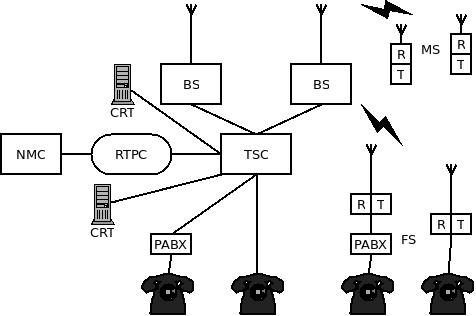
\includegraphics[width=\textwidth]{Imagen/diaPMR.jpg}
\caption{Estructura de un sistema PMR  multiemplazamiento}
\label{img:diaPMR}
\end{figure}
% subsubsection PMR (end)
\subsubsection{Sistemas PMR: Sistemas troncales}
\label{ssub:troncales}
	Son sistemas de concentración de enlaces, en donde la asignación de frecuencias a los usuarios es dinámica. Son sistemas en espera y se utiliza la función Erlang-C para su dimensionamiento. Por su necesidad de dinamismo es necesario un sistema de señalización para la asignación de canales y la gestión de las colas de llamadas. Para la señalización se suele utilizar un protocolo ALOHA ranurado con longitud de trama variable.\\
	
% subsubsection troncales (end)